\chapter{Anforderungen und Analyse}\label{kap:anforderunganalyse}

\section{Ziel der Arbeit}\label{sec:zielderarbeit}


Wie in der Einleitung \ref{kap:einleitung} beschrieben, soll 
ein CNN Basiertes System zur Wildtiererkennung entwickelt 
werden, das für dir Inferenz den Neural Compute Stick 2 verwendet.
Dabei sollte neben der reinen Erkennung auch eine Lokalisierung 
der erkannten Tiere im Bild stattfinden. Gängige Techniken dafür 
werden im nächsten Abschnitt erläutert.
\\
Anforderungen an die Erkennung waren ein möglichst hohe 
Genauigkeit und Robustheit des Models zu schaffen, sodass 
diese auch für die weniger detailreichen graustufen Bilder 
der Infrarot kamera noch funktioniert. Echtzeit Inferenz 
war nicht notwendig, dennoch sollten alle relevanten Informationen 
verarbeitet werden können.
\\
Die entwicklung der autonome laufenden Anwendung für den Raspberry, 
sowie die Integration des trainierten Modells in diese war ebenso 
wichtigier Bestandteil der Arbeit.
\\
Hierbei waren die anforderungen eine geeignete Kamera (infrarot) 
auszusuchen, sowie eine Kommunikations/Benachrichtigungs 
möglichkeit über Netzwerk verbindung zu schaffen.


\section{Related Work}\label{sec:related_work}

Für die Objekterkennung werden häufig End-to-End Lösung verwendet,
Modelle die sowohl Klassifikation als auch Lokalisierung 
durchführen.
Diese verwenden meist eines der im Abschnitt 
\ref{subsubsec:architecture} aufgezeigten Basis CNNs als  
Feature Extractor und darauf aufbauend ein Framework für die 
Lokalisierung. 


Diese lassen sich in einstufige und zweistufige Verfahren 
gliedern \cite{wengObjectDetectionPart2018}. Bei den zweistufigen
handelt es sich um Regionbased CNNs, die Regionen für
mögliche Box Locations mithilfe RPN (Region Proposia Network)
oder selective search verfahren finden soll, um diese dann
zu klassifizieren bzw box regression. Die aktuellste Version 
davon ist das in Abbildung \ref{fig:faster_rcnn} schematisch 
dargestellte \textit{Faster R-CNN} \cite{renFasterRCNNRealTime2016a}


Einstufige Verfahren wie Single Shot Detectoren (SSD) 
führen die lokalisierung zusammen mit dem Feature Extractor 
aus, indem verschiedene scalierungen/ausmaße der Convolutional 
Layer in den Classifier/Regressor gegeben werden.
Dadurch sind diese wie in Abbildung \ref{fig:speed_acc}
zu erkennen ist, zwar schneller, jedoch auch ungenauer.

\begin{minipage}[t]{0.5\textwidth}
    \centering
    \label{fig:faster_rcnn}
    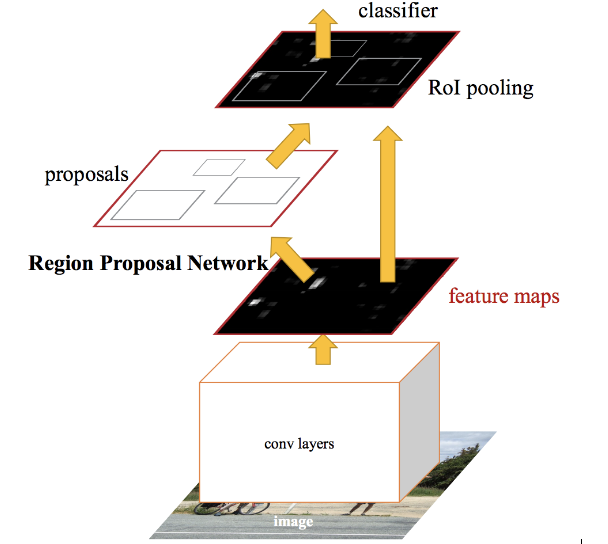
\includegraphics[width=0.67\textwidth]{faster_rcnn.png}
    \captionof{figure}{Faster R-CNN, \cite{renFasterRCNNRealTime2016a}}
\end{minipage}
\begin{minipage}[t]{0.5\textwidth}
    \centering
    \label{fig:speed_acc}
    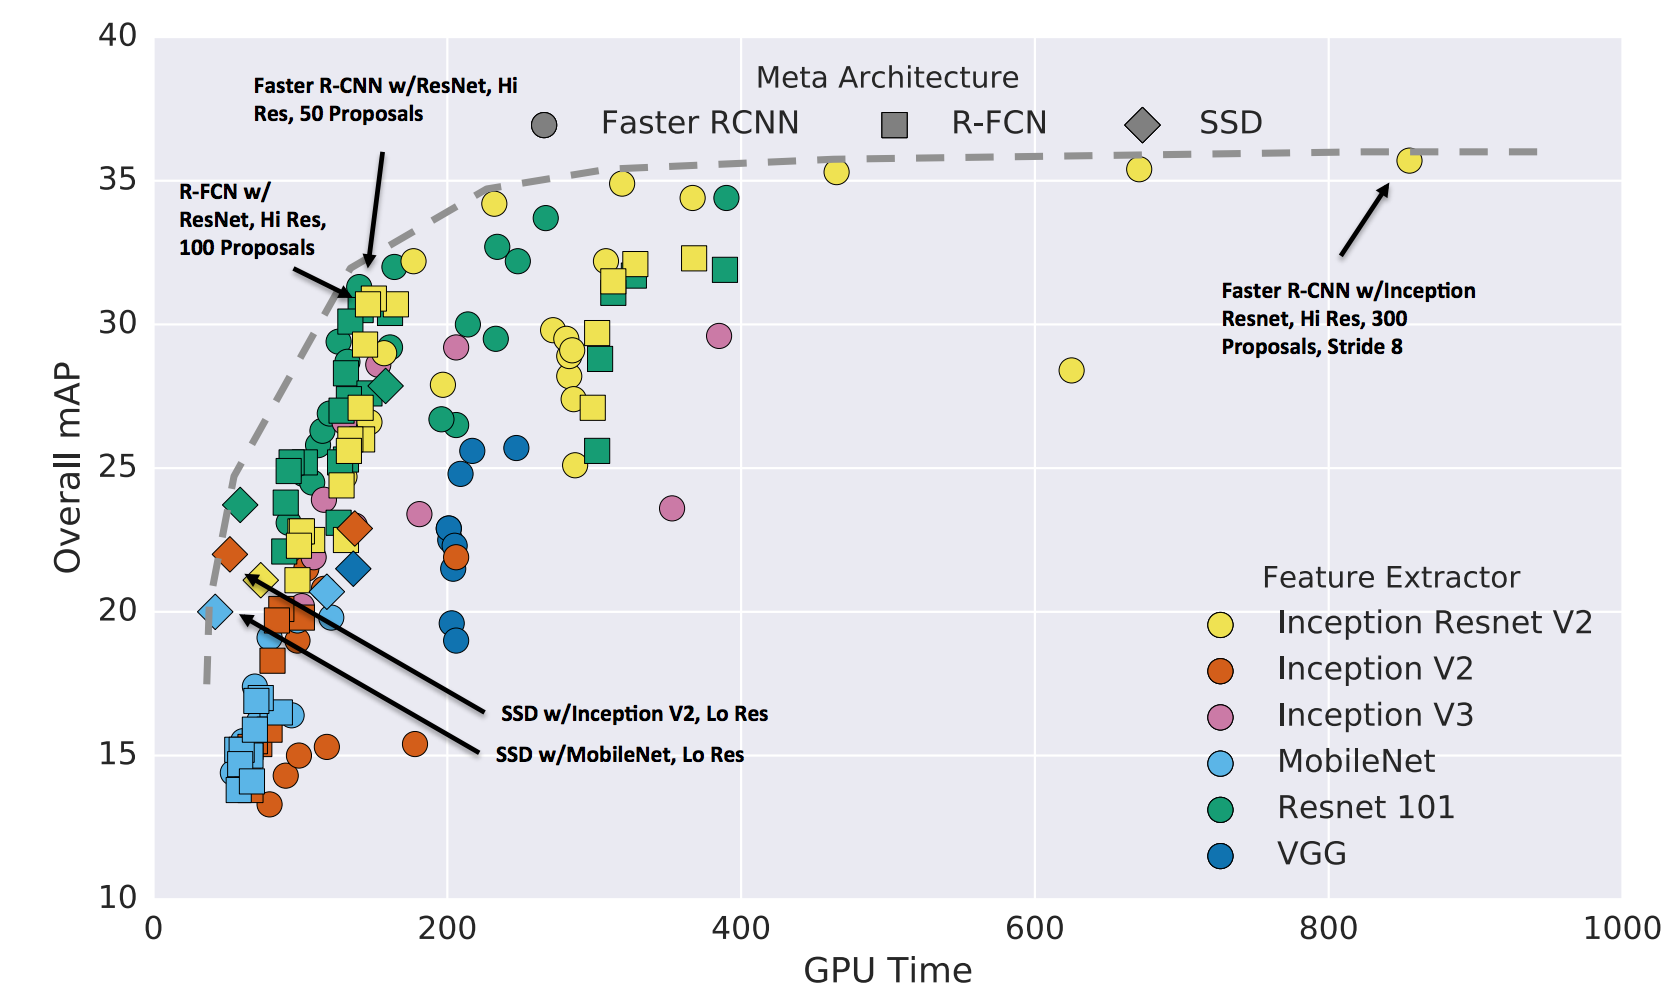
\includegraphics[width=\textwidth]{speed_acc_comp.png}
    \captionof{figure}{Geschw vs Genauigkeit, \cite{huangSpeedAccuracyTradeOffs2017}}
\end{minipage}

